\section{Motivation and Background  \label{background}}
\subsection{Motivation}
As we mentioned in the section \ref{intro}, a key goal of our efforts  is to develop methods to use DL to help predict properties of molecules from first principles. That is, rather than trying to engage in complex and often {\em intuition-based} feature engineering efforts that require experienced domain scientists, we want to use basic and readily available chemical and physical information as input to the models. The rationale behind this is that deep neural networks have been shown to excel at using early layers in the network as {\em feature generators} that are then used by mid and late layers in the network. Properly trained and tuned deep models have been shown to rival or surpass  human ability in domains such as language translation and computer vision (REFS). Thus, a successfully trained model that is based on first principle data can help a wider range of scientists and practitioners study and predict properties of novel molecules. 

Publicly available databases, such as PubChem (REF) and OQMD (REF) provide the foundational information from which to draw the set of basic features to serve as input  to the model. These databases provide a) chemical properties, b) physical properties, c) 2D and 3D imaging on spatial structures of molecules,  and d) 2D imaging on molecular spectroscopy, to name a few.

\subsection{Problem Formulation}
We can state our problem as follows. Supposed we have a data set $\mathcal{S}$, consisting of a collection of records $s_0, s_1, ..., s_n$ containing information about some group of molecules. Let $\mathcal{P} = \{p_0, p_1, ..., p_r\}$ be a collection of molecular properties that we want to predict or estimate from $\mathcal{S}$.  Our task is to: 
\begin{enumerate}
	\item Transform $\mathcal{S}$ into an input data set $X = \{x_0, x_1, ..., x_m\}$, where each element $x_i$ is an example that represents 
	some set of properties extracted from an item $s_j \in  \mathcal{S}$. In this case, each example $x_i$ is a multi-dimensional vector and 
	$X$ is a matrix containing these examples.
	\item Define one or more deep learning models $M_0, M_1, ... M_p$ that predict the properties in $\mathcal{P}$. Thus, the prediction $y$ for a given model $M_k$ might contain one or more of the properties in $P$. In other words, in theory, the prediction $y$ can be a multi-dimensional vector $y = \{y_0, y_1, ..., y_l\}$ , $l \leq r$, where each component represents some property in $\mathcal{P}$. For simplicity, in this paper we only consider models that predict one property at time,  from the input data $X$. Hence the model's output is one-dimensional
	\item Use $X$ to train one or more deep learning models $M_0, M_1, ... M_p$. For each $x_i$ in $X$, a given model $M_k$ will output a prediction $y_i$. The collection of predictions $y_0, y_1, ..., y_m$ forms a column vector $Y$. 
\end{enumerate}
Thus, we have established the basic framework to handle the task of molecular property prediction as a regular machine learning problem. 
\subsection{PubChem Database}
The PubChem\footnote{PubChem URL: https://pubchem.ncbi.nlm.nih.gov} Database is one of the largest databases of chemical molecules and their properties. PubChem is freely available and is maintained by the National Library of the Medicine of the U.S. National Institutes of the Health (NIH). The database contains hundreds of millions of entries and provide search capabilities based on the name of the chemical, its molecular formular, or its compound identifier.  Programatic access to  PubChem is available through PUG-REST (REF), a Python-based REST API. 

For the purpose of this paper, we shall focus on a sub-set of PubChem that contains the following basic molecular properties:
\begin{enumerate}
	\item {\em CID} - unique compound identifier within PubChem. This a nine-digit numeric string. 
	\item {\em Molecular Formula} -  a string that specifies the type and number of atoms in a molecule. For example, the molecular formula for the widely-used analgesic acetaminophen is C8H9NO2.
	\item {\em Canonical SMILES} - a string that specifies the chemical structures and bonds in a molecule. For example, the Canonical SMILES string for acetaminophen is CC(=O)NC1=CC=C(C=C1)O. We shall discuss more about the SMILES notation is section \ref{smiles}.
	\item {\em Isomeric SMILES} - a variation of the SMILES notation that includes isomers - molecules with identical molecular formula but different arrangement of its constituents atoms in space. The Isomeric SMILES for acetaminophen is [2H]C1=C(C(=C(C(=C1NC(=O)C)[2H])[2H])O)[2H].
	\item {\em Molecular Weight} - this is real number that represents the mass of a given molecule and its measured in {\em daltons}, or in molar mass (g/mol). The molecular weight for acetaminophen is 155.19 g/mol.
	\item {\em XLogP} - this is real number representing the logarithm of the partition coefficient $\boldsymbol P$ of the molecule with respect to 1-octanol and water, and computed with the XLogP3 method. 
\end{enumerate}
PubChem has many more data elements, and we encourage the interested reader to further explore this comprehensive database. 

\subsection{SMILES Representations\label{smiles}}
The Simplified Molecular Input Line Entry System (SMILES) is a character-based line notation for describing chemical structures in a way that is easier for computers to interpret. SMILES strings can be mapped into two-dimensional or three-dimensional models of the spatial organization of the atoms in the molecules being represented by the string. The notation consists of a series of characters containing no spaces that uses a simple vocabulary and a few grammar rules. In this notation atoms are represented by their atomic symbol while bonds and branches are represented by special characters. Figure \ref{fig:cyclamic}, obtained from PubChem,  shows the 2-D chemical structure depiction for the compound Cyclamic acid. The molecular formula for this compound is C6H13NO3S, and its canonical SMILES representation is C1CCC(CC1)NS(=O)(=O)O.

\begin{figure}[htb]
        \centering
        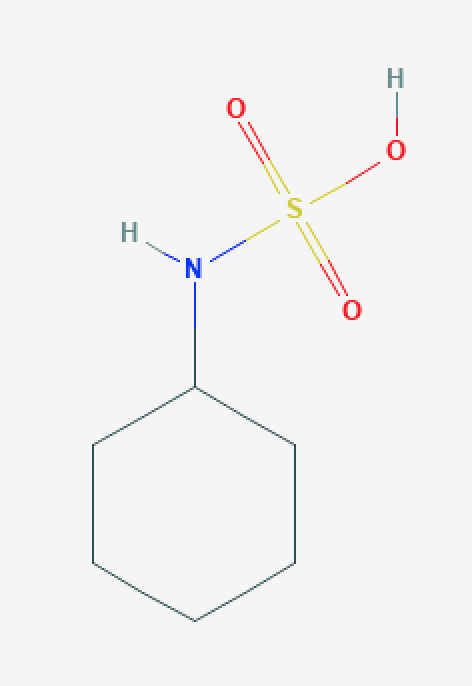
\includegraphics[width=0.20\textwidth]{figures/cyclamic_acid.png}
        %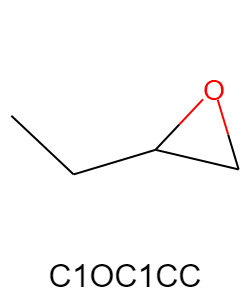
\includegraphics[width=0.25\textwidth]{figures/Smiles-Smile2.png}
        \caption{2-D chemical structure of Cyclamic acid.}
        \label{fig:cyclamic}
    \end{figure}
    
One complication with SMILES is that straightforward application of the basic rules for generating a SMILES string can yield more than one string representation per molecule. To solve this, some {\em canonicalization} algorithm is typically used in chemical databases to  assign just one representation per structure and permit consistency. In PubChem, this representation is called {\em Canonical SMILES}. 
{\em Isomeric SMILES} are a variation of SMILES in which information on isotopes and stereochemistry (i.e., 3-D structures) is included within the string. A detailed description of the specifics of these canonicalization algorithms, isomeric variations, and stereochemistry is beyond the scope of this paper (REF). The original SMILES framework was a proprietary framework, but since them new open-standard called OpenSMILES\footnote{OpenSMILES URL: http://opensmiles.org/} has been developed by the chemistry research community.
%
%    \begin{itemize}
%        \item Simplified Molecular Input Line Entry System (SMILES) is a line notation for describing chemical structures in a way that is easier for computers to interpret. 
%        \item It consists of a series of characters containing no spaces that uses a simple vocabulary and a few grammar rules.
%        \item In this notation atoms are represented by their atomic symbol while bonds and branches are represented by special characters.
%        \item Unfortunately based exclusively on the basic rules for generating a SMILES string there can exist more than one way to represent a single compound.
%        \item To help assign just one representation per structure and permit consistency a canonicalization algorithm is typically used by databases. This algorithm's job is to generate and assign one specific SMILES string for each structure.
%        \item In our dataset these are called canonical SMILES.
%        \item Another type of SMILES string that are often used and are also available in our dataset are isometric SMILES. These include isotopic specifications of a chemical structure.
%    \end{itemize}
    \subsubsection{SMILES Rules}
    In this section we provide a short overview on how SMILES encode structural information of molecules. For a more detailed treatment, the interested reader is referred to the full OpenSMILES specification. Figure \ref{fig:smile-examples} will be used to illustrate some of these concepts.
    
        \begin{figure}[htb]
        \centering
        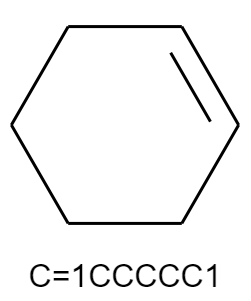
\includegraphics[width=0.25\textwidth]{figures/Smiles-Smile1.png}
        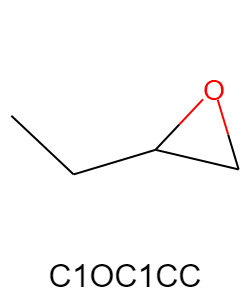
\includegraphics[width=0.25\textwidth]{figures/Smiles-Smile2.png}
        \caption{Example of 2 chemical structures and their respective SMILES}
        \label{fig:smile-examples}
    \end{figure}

    Basic rules: 
    
%    Atoms are represented by their atomic symbol and are enclosed in brackets []. The organic subset can be written without brackets, these include: B, C, N, O, S, F, Cl, Br, and I. Brackets can also be used to remove ambiguities about the charge of the atom. Bonds are represented as follows: 1) $-$ : single bond, 2) $=$ :  double bond, 3) $\#$ : triple bond, and 4) $.$ : disconnected structure.
        \begin{enumerate}
            \item Atoms are represented by their atomic symbol and are enclosed in brackets []. The organic subset can be written without brackets, these include: B, C, N, O, S, F, Cl, Br, and I. Brackets can also be used to remove ambiguities about the charge of the atom. 
            \item Bonds are represented as follows: 
            \begin{itemize}
                \item[$-$] single bond.
                \item[$=$] double bond.
                \item[$\#$] triple bond.
                \item[$.$] disconnected structure.
            \end{itemize}
            \textbf{Note:} Single bonds can be omitted as shown in the example for  Cyclamic acid, and in Figure \ref{fig:smile-examples} .  This is typically done with the atoms in the organic subset.  %and \ref{fig:smile-examples2}.
            \item Branches are represented with parenthesis ().
            \item Cyclic structures or carbon rings are represented with digits. The first digit is the beginning of the rings and the matching digit that follows is when the ring closes. This can also be observed in Figures \ref{fig:smile-examples} and \ref{fig:smile-examples2}.
        \end{enumerate}
    \subsubsection{Correspondence between the 2D structure and a SMILES}
        \begin{itemize}
            \item In Figure \ref{fig:smile-examples} we can see two chemical models each with a cyclic cycle.
            \item Each edge and end of the 2D model represent a carbon and in both the model and SMILES the hydrogen is omitted as it is assumed that they fill any missing bonds.
            \item Notice in Figure \ref{fig:smile-examples} the leftmost figure its SMILES has a double bond which is illustrated in the 2D model. It is then followed by a digit indicating that the next sequence is for a cyclic structure. 
            \item So in this first figure we have that it starts at a carbon which is the starting point for a cyclic cycle and the cycle starts with a double bond. 
            \item In the rightmost image we see similarly that it starts with a carbon, in this case it is the one located at the leftmost edge of the triangle. This carbon starts the cycle that includes an oxygen atom and note that when the cycle closes the next part of the SMILES continues from the initial carbon.
            \item In Figure \ref{fig:smile-examples2} we can observe a more detailed example that better illustrates how the various rules come together to represent what we see in the 2D model.
            \item The initial red 'C' in the SMILES is shown in the 2D structure with the red circle. That is our starting position. 
            \item This is followed by a '1' implying that the red 'C' belongs in a carbon ring and will be treated as the starting point of it. And the carbon ring closes at the orange 'C' since this is followed by the second '1'.
            \item We can notice as well that the orange 'C' also forms part of a branch as it is enclosed in a parenthesis. The entire branch can be observed in the 2D model inside the purple circle.
            \item Finally the green text of the SMILES can be seen inside the green circle. Notice that it is attached to the first carbon of the SMILES (red 'C'). 
        \end{itemize}
    
    \begin{figure}[h]
        \centering
        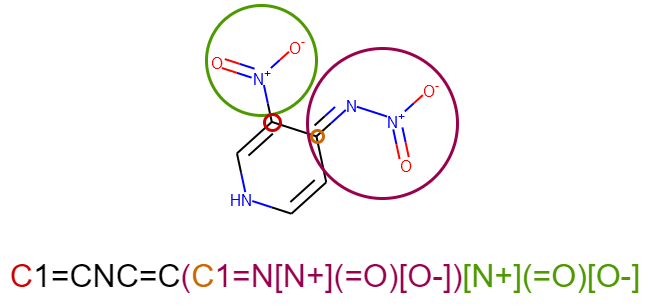
\includegraphics[width=0.5\textwidth]{figures/Smiles-Smile3.png}
        \caption{Example of how each part of the SMILES string corresponds to the 2D model of the chemical structure.}
        \label{fig:smile-examples2}
    \end{figure}
\subsection{Applying NLP Ideas}
